%\clearpage
\section{Робот Self Balancing Robot}
\subsection{Обзор робота}
Самобалансирующийся робот представляет собой сложную систему управления с замкнутым контуром
, которая автономно балансирует себя на месте. Он собирает обратную
связь с нескольких датчиков, включая встроенный акселерометр
myRIO, гироскоп и датчики, встроенные в оба двигателя. Он использует
дополнительный фильтр и PD (пропорционально-дифференциальный) контроллер
в LabVIEW, чтобы стоять вертикально.

\subsection{Описание робота}
Колеса вращаются двигателями постоянного тока, которые работают
независимо и получают данные ШИМ для управления их скоростью.
Датчики, встроенные в каждый двигатель, измеряют относительное
положение и связываются с myRIO с помощью специализированных
цифровых линий кодирования.
Встроенный трехосевой акселерометр myRIO измеряет
статическое и динамическое ускорение.
Гироскоп измеряет скорость вращения и
взаимодействует с myRIO по
протоколу связи I2C.
Дополнительный фильтр используется для обработки данных акселерометра и гироскопа для устранения высокочастотного шума
акселерометр и низкочастотный шум гироскопа.
Регулятор PD используется для управления положением двигателя относительно друг друга.
MyRIO подключается к \\
хост-компьютеру через Wi-Fi.

\newpage
\subsection{Сборка робота}
\begin{figure}[h!]
    \begin{subfigure}[b]{0.45\textwidth}
        \centering
        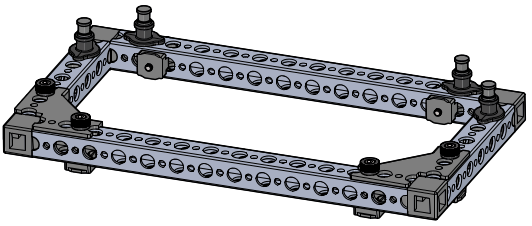
\includegraphics[width=0.7\textwidth]{fig/assembly/3.1.png}
        \caption*{Шаг 1}
    \end{subfigure}
    \begin{subfigure}[b]{0.45\textwidth}
        \centering
        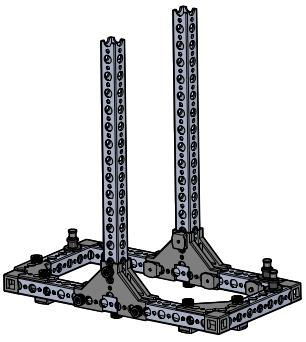
\includegraphics[width=0.7\textwidth]{fig/assembly/3.2.png}
        \caption*{Шаг 2}
    \end{subfigure}
    \begin{subfigure}[b]{0.45\textwidth}
        \centering
        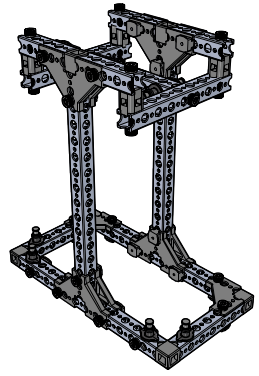
\includegraphics[width=0.7\textwidth]{fig/assembly/3.3.png}
        \caption*{Шаг 3}
    \end{subfigure}
    \begin{subfigure}[b]{0.45\textwidth}
        \centering
        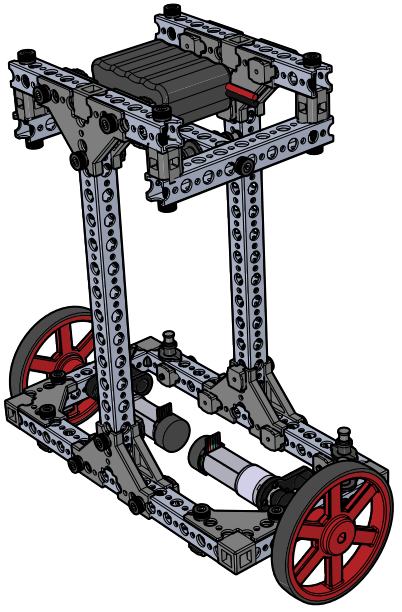
\includegraphics[width=0.7\textwidth]{fig/assembly/3.4.png}
        \caption*{Шаг 4}
    \end{subfigure}
    \begin{subfigure}[b]{0.45\textwidth}
        \centering
        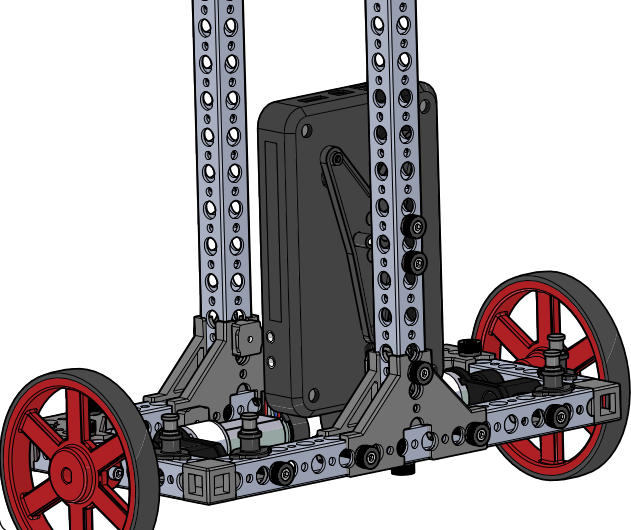
\includegraphics[width=0.7\textwidth]{fig/assembly/3.5.png}
        \caption*{Шаг 5}
    \end{subfigure}
    \begin{subfigure}[b]{0.45\textwidth}
        \flushright
        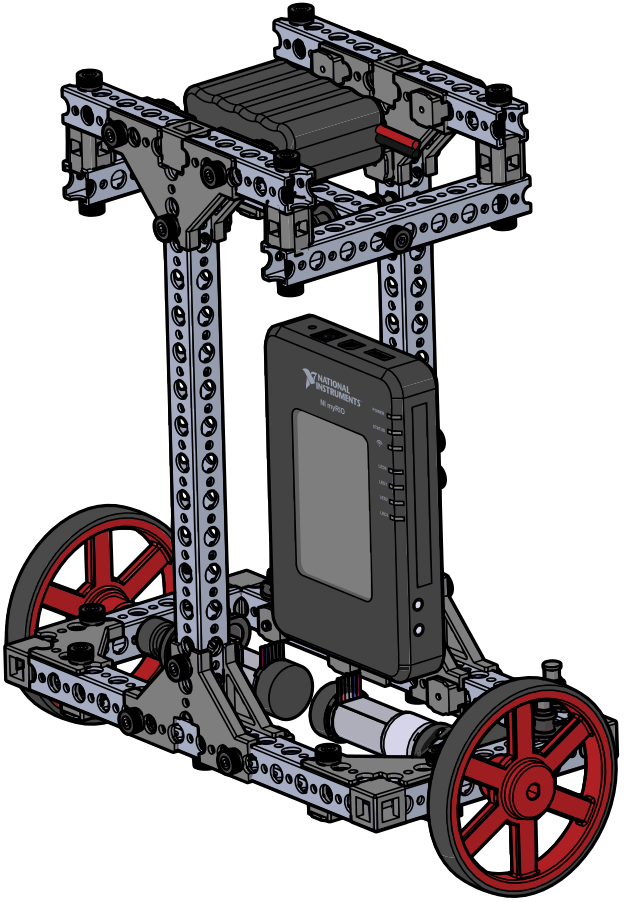
\includegraphics[width=0.7\textwidth]{fig/assembly/3.6.png}
        \caption*{Шаг 6}
    \end{subfigure}
\end{figure}
\clearpage

\newpage
\subsection{Подключение робота}
Подключение робота представлено на рисунке \ref{3connect}.
\begin{figure}[h]
    \centering
    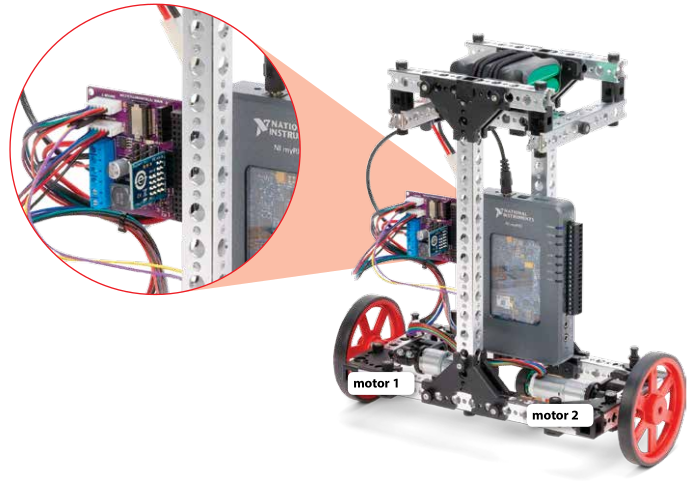
\includegraphics[width=0.5\textwidth]{fig/assembly/3.7.png}
    \caption{Подключение двигателей и периферии}
    \label{3connect}
\end{figure}

\subsection{Испытание робота}
Самобалансирующийся робот и два зубчатых колеса с приводом от двигателя постоянного тока являются установкой и исполнительными механизмами соответственно. Набор датчиков
включает в себя гироскоп, который измеряет угловую скорость, и акселерометр, который измеряет негравитационное
ускорение. Поскольку известно, что акселерометр и гироскоп имеют систематические ошибки и зашумлены,
сигналы от датчиков объединяются для получения точного измерения угла ориентации робота —
более точного, чем может быть достигнуто с помощью любого датчика по отдельности. Команды внешней ссылки вводят
Цель конструкции - уравновесить робота в вертикальном
положении при наличии внешних помех и обеспечить его надежную устойчивость к колебаниям растений. Контроллер - это контроллер PD.
Управляющая программа робота представлена на рисунке \ref{3prog}.
\begin{figure}[h]
    \centering
    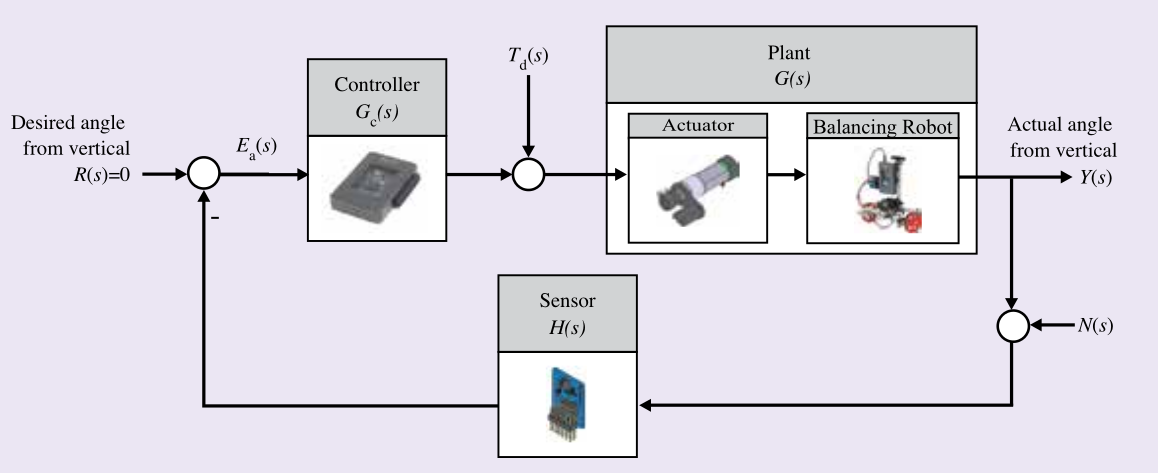
\includegraphics[width=0.4\textwidth]{fig/assembly/3.8.png}
    \caption{Управляющая программа робота}
    \label{3prog}
\end{figure}

%\subsection{Устранение неисправностей}
%\begin{itemize}
%    \item Дважды проверьте, правильно ли подключены двигатели и энкодер -- если их поменять местами, робот не будет балансировать
%    \item Если вы возьмете в руки самобалансирующегося робота или нажмете на него слишком сильно, то может сбиться калибровка. Для возвращения робота в рабочее состояние проведите повторную калибровку. Нажмите кнопку 0 в нижней
%    части myRIO, чтобы выключить колеса и систему управления, а затем проведите калибровку, чтобы снова сбалансировать его. Процедура калибровки выглядит следующим образом:
%    \begin{itemize}
%        \item Держите робота вертикально так, чтобы его центральная линия была перпендикулярна земле
%        \item Нажмите <<Button 0>> в нижней части myRIO, все еще удерживая робота вертикально, и быстро отпустите
%    \end{itemize}
%\end{itemize}